\section{BaconBits Hardware}

\begin{frame}
   {Component Placement}

	     \begin{figure}[H]
		     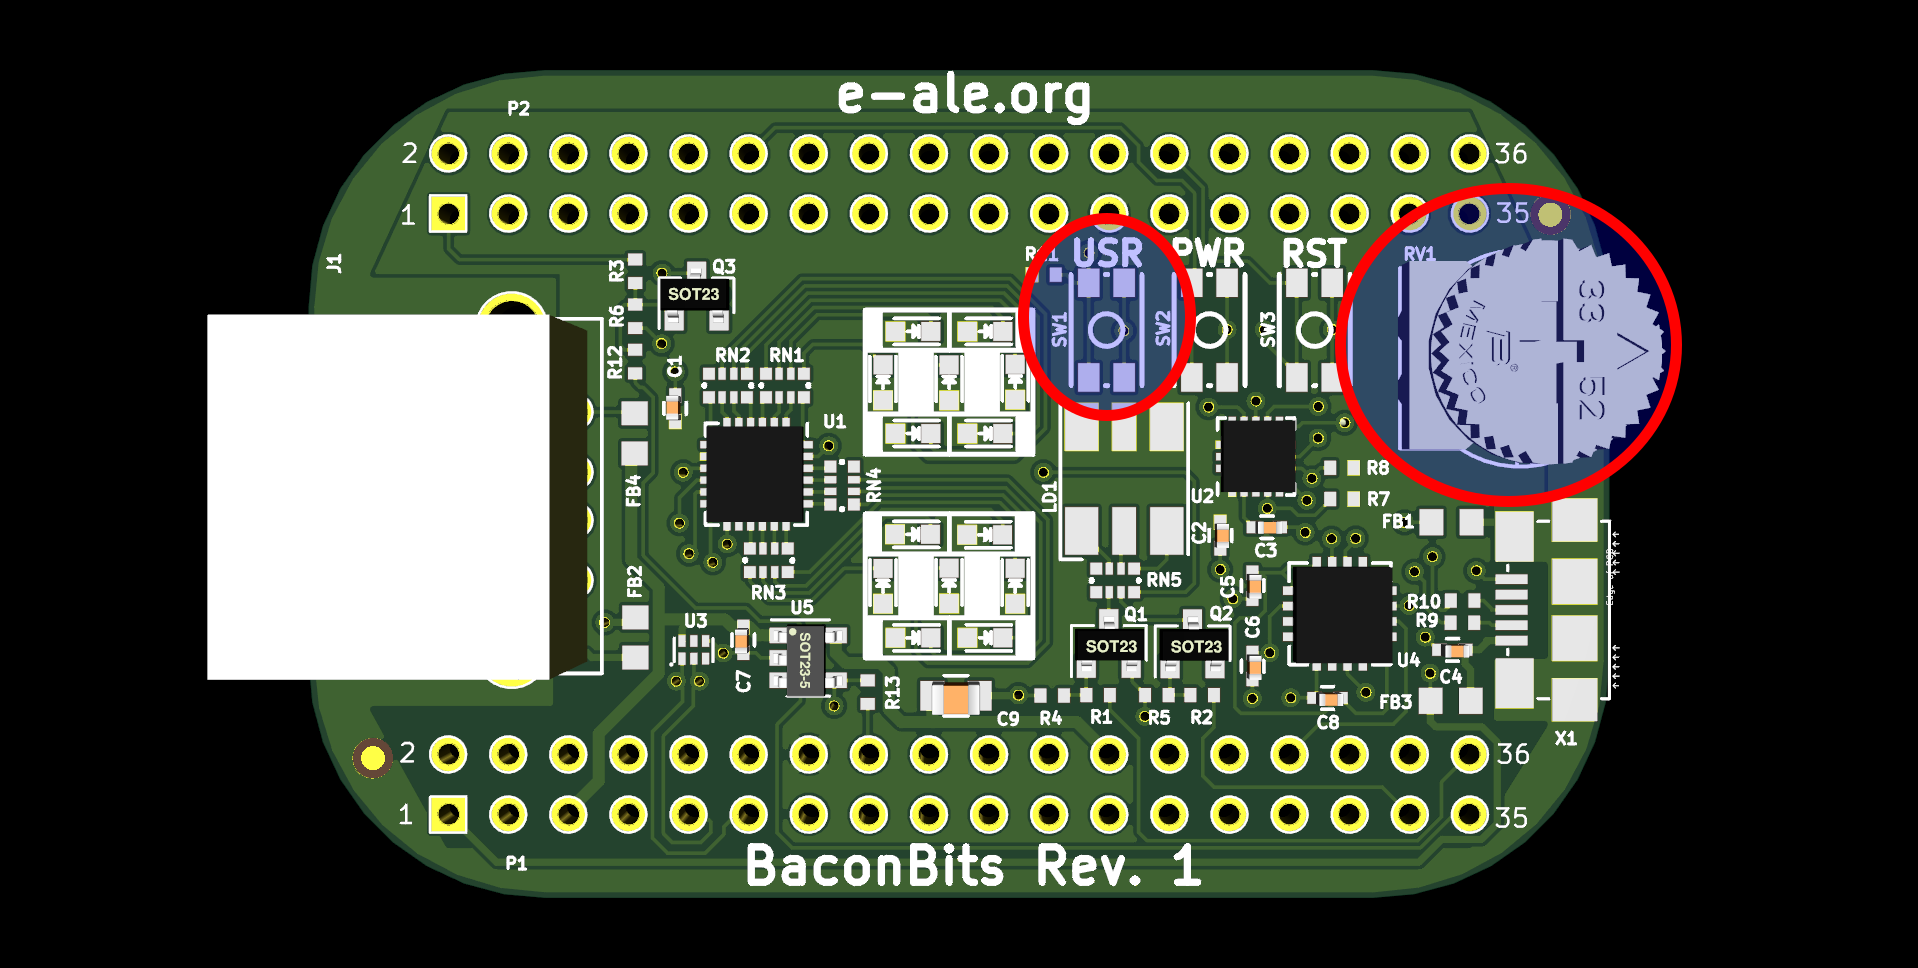
\includegraphics[width=5in]{IMAGES/baconbits-mech-annotated}
				       \caption{BaconBits Component Identification}
	     \end{figure}
   \begin{itemize}
      \item
	      \textbf{RV1} is the thumbwheel device
   \end{itemize}
\end{frame}

\begin{frame}
	{BaconBits Schematic Overview}
	\begin{itemize}
		\item
			\url{https://github.com/e-ale/BaconBitsCapeHW/blob/master/baconbits.pdf}
	\end{itemize}


	     \begin{figure}[H]
		     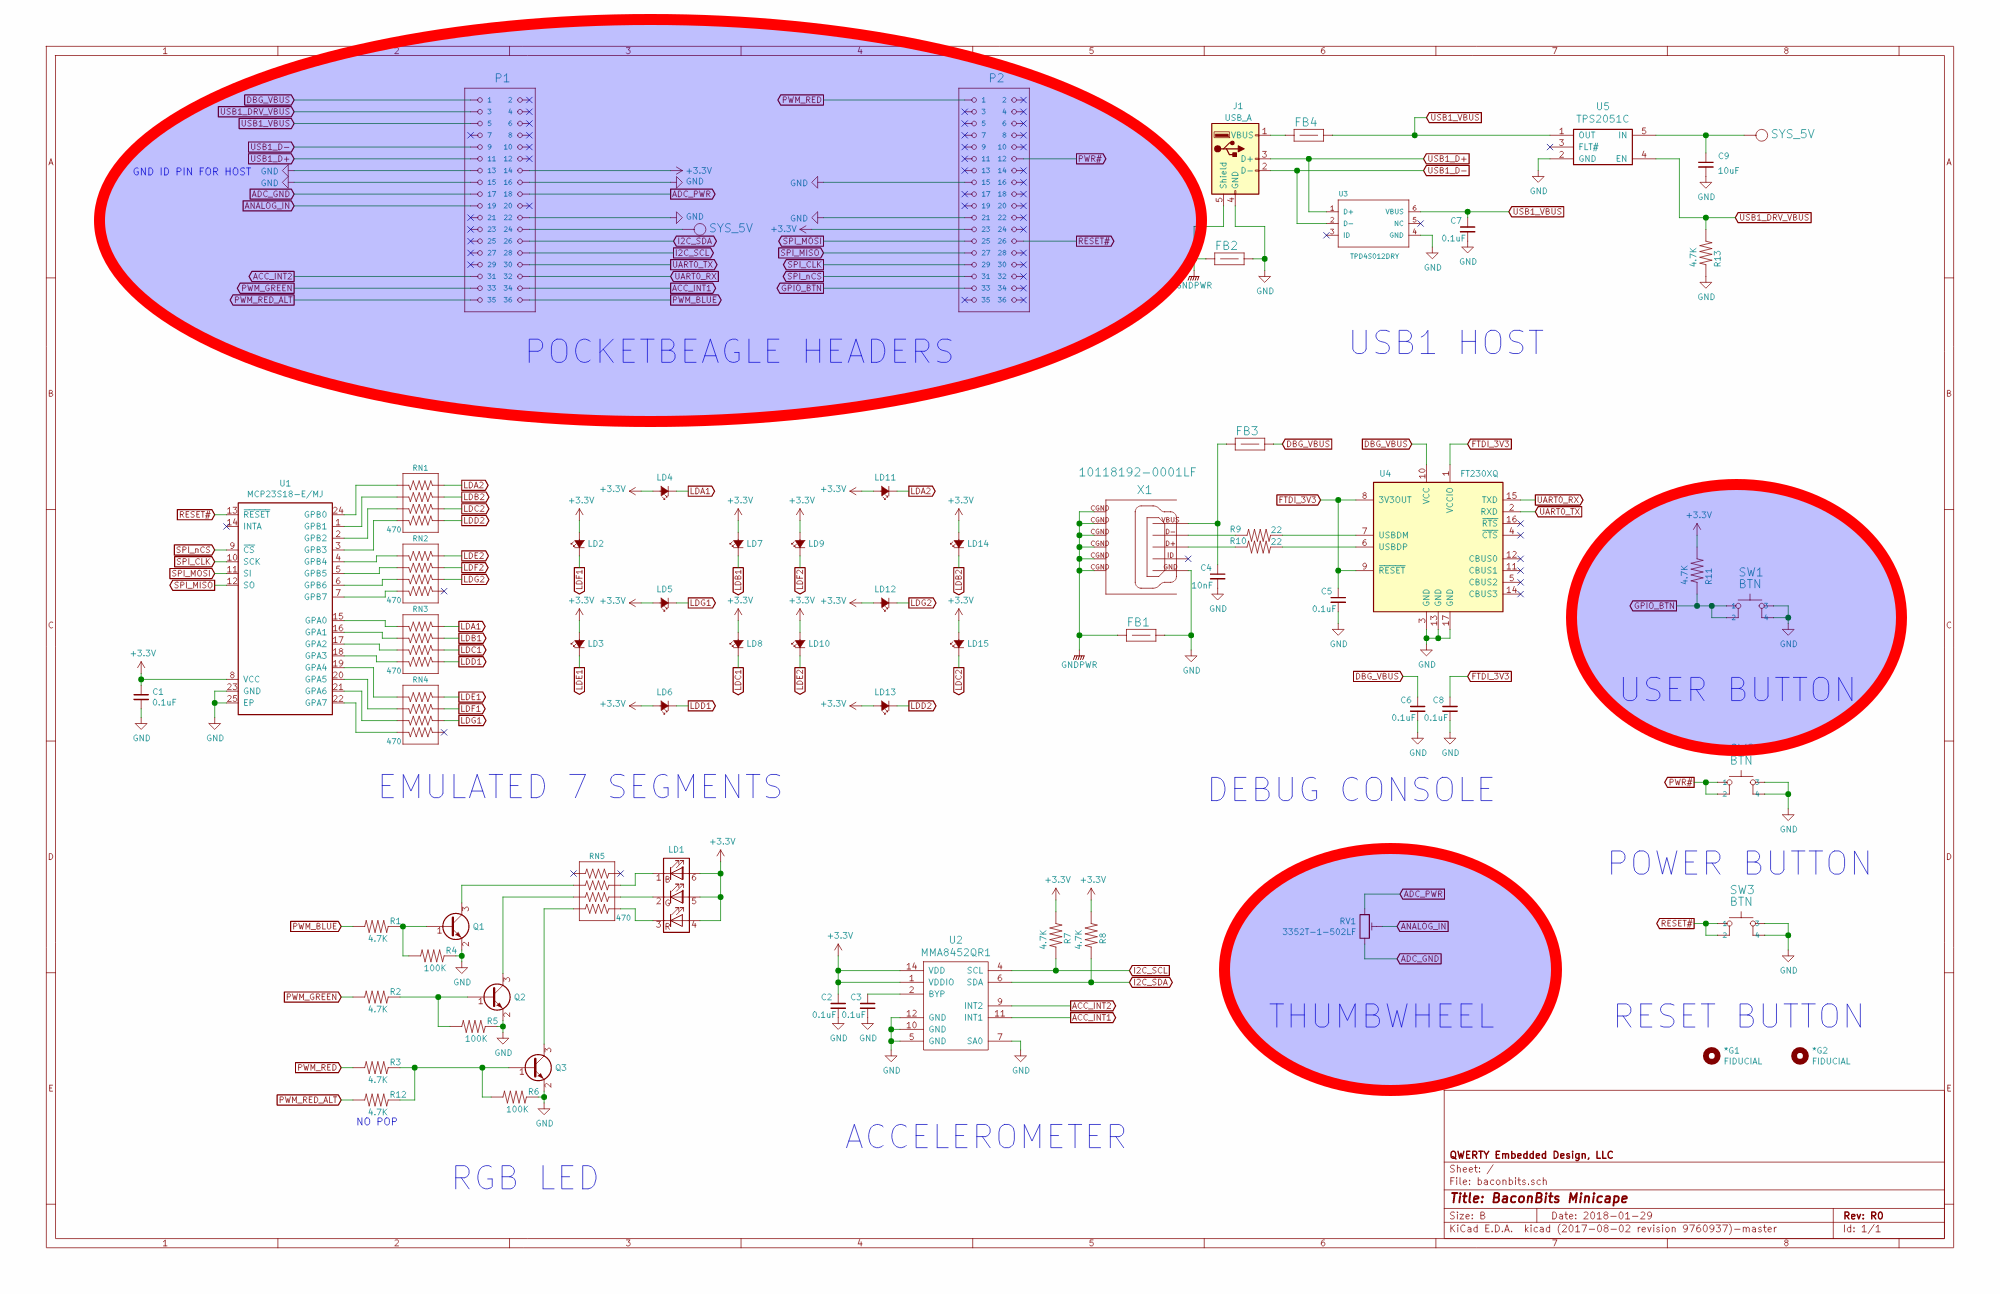
\includegraphics[width=5in]{IMAGES/baconbits-schematic-annotated}
				       \caption{BaconBits Schematic}
	     \end{figure}
\end{frame}

\begin{frame}
	{BaconBits Thumbwheel}
	     \begin{figure}[H]
		     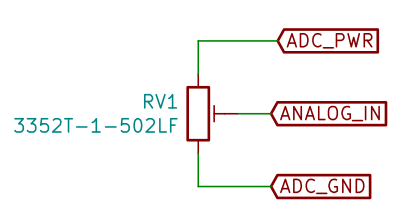
\includegraphics[width=3in]{IMAGES/baconbits-thumbwheel}
				       \caption{BaconBits Thumbwheel}
	     \end{figure}
	     \begin{itemize}
		     \item
		Signals:
	\begin{itemize}
		\item
			\textbf{ADC\_GND}
		\item
			\textbf{ADC\_PWR}
		\item
			\textbf{ANALOG\_IN}
	\end{itemize}
	\end{itemize}


\end{frame}

\begin{frame}
	{BaconBits P1 Connector}
	     \begin{figure}[H]
		     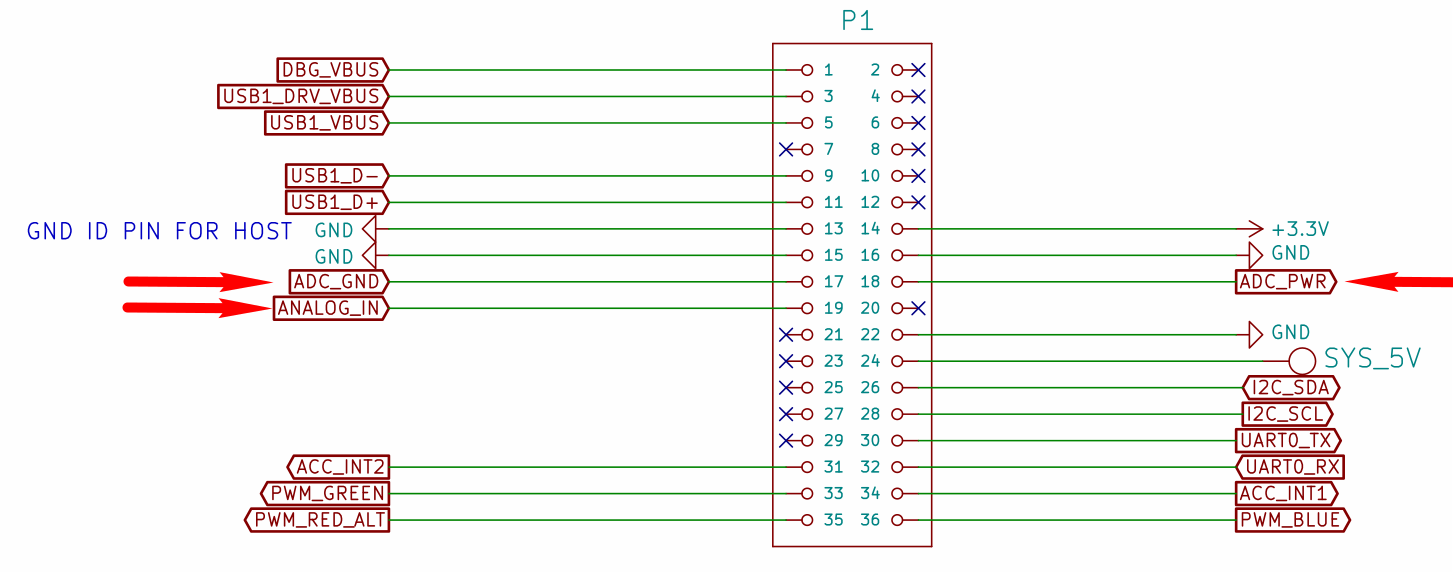
\includegraphics[width=4.5in]{IMAGES/baconbits-p1-annotated}
				       \caption{BaconBits P1 Connector}
	     \end{figure}
	     \begin{itemize}
		     \item
		Pins:
	\begin{itemize}
		\item
			\textbf{ADC\_GND : P1-17}
		\item
			\textbf{ADC\_PWR : P1-18}
		\item
			\textbf{ANALOG\_IN : P1-19}
	\end{itemize}
	\end{itemize}
\end{frame}
